%!TeX root = ./../MusterAbschlussarbeit.tex

%##########################################################
% Inhalt
%##########################################################

\clearpage
\chapter{Theoretische Grundlagen}
\section{Neuronale Netze}
Neuronale Netze sind ein Modell für künstliche Intilligenz nach vorbild des Gehirns.
Es besteht aus mehreren Schichten verknüpften Neuronen, welche numerische Informationen verarbeiten und in einen Output umwandeln. Die Ausgänge der vorderen Neuronen sind dabei immer mit den Eingängen der Neuronen der nächsten Schicht verknüpft.
Jedes Neuron besitzt eine Aktivierungsfunktion, welche entscheidet ob es aktiv ist oder nicht. Neuronen geben werte von 0 (passiv) bis 1 (aktiv) an dahinterliegende Neuronen.

Richtig trainierte Neuronale Netze können gute Antworten für komplexe Problemstellungen geben, so liefern sie beispielsweise in der Mustererkennung gute Ergebnisse.

[Ertel ~S. 290]
\subsection{Training von NN}

Wird ein NN initialisiert werden Kantengewichte zwischen den Neuronen zufällig verteilt. Diese Kantengewichte sorgen dafür wie stark einzelne Neuronen in die nachfolgende Rechnung eingehen.
Deshalb liefern untrainierte NN schlechte Ergebnisse und müssen trainiert werden, bevor sie Problemstellungen richtig lösen können.

Während des Trainings eines NN werden Kantengewichte angepasst um die Heuristik  an ein optimales Ergebnis anzupassen.

Für das Training von NN wird viel Rechenleistung gebraucht, da der Prozess mit sehr vielen Rechenoperationen verbunden ist.

[Ertel ~S. 290]
[Quelle?]
\section{Reinforcement Learning}
Reinforcement Learning ist ein Bereich des maschinellen Lernens, bei welchem ein Agent durch Interaktion mit seiner Umgebung lernt, welche Aktionen in welchen Situationen am besten geeignet sind um ein bestimmtes Ziel zu erreichen.
Da ein Agent keine konkrete Vorgehensweise besitzt, versucht er über Trial-and-Error herrauszufinden welche Aktionen zu Belohnungen führen.

\subsection{Agent und Umwelt}
Bestandteile des RL sind der Agent und die Umwelt. Der Agent bekommt die Informationen der Umwelt übergeben und entscheidet welche Handlungen daraus folgen sollen.
Das Environment setzt die Aktionen des Agenten in Hanldungen um und bewertet diese mit numerischen Rewards, welche als Belohnung fungieren.
Anhand der erhaltenen Rewards, versucht der Agent seine Aktionen anzupassen um die zukünftigen Belohnungen zu maximieren.

\newpage
\subsection{Markov- Entscheidungsprozess}
Jedes RL Problem lässt sich durch den Markov Entscheidungsprozess (Markov decision Prozess) beschreiben.
Der MLP ist ein mathematisches Modell für Entscheidungsprobleme, bei welchem der Agent abhängig von der Umwelt entscheidungen trifft um ein bestimmtes Ziel zu erreichen.
MDP setzen die Einhaltung der Markov-Eigenschaft vorraus. Diese ist erfüllt, wenn ein Zustandsübergang nur vom letzten Zustand und der letzten Aktion abhängig ist.
Die Abbildung1 stellt den Ablauf eines MDP dar.


Hauptkomponenten des MDP:
\setlist{noitemsep}
\begin{itemize}
\item endliche Menge valider Zustände
\item endliche Menge valider Aktionen
\item Belohnungsfunktion
\item Verhaltensstrategie
\end{itemize}




\begin{figure}[!htb]
	\centering
	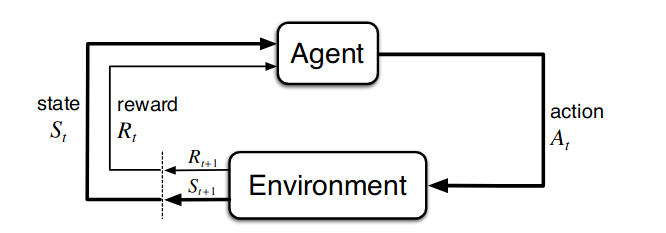
\includegraphics[width=0.7\textwidth]{Bilder/Markov.png}
	\caption{Quelle:Einstieg DeepLearning Zai/Brown S27}
\end{figure}

\subsection{Zustände, Aktionen, Verhaltensstrategie und Belohnungen}
Ein RL-Agent nimmt seine Umgebung als eine Menge an bestimmten Zuständen war.
Jeder Zustand enthält eine Vielzahl von Merkmalen und Eigenschaften welche für die Entscheidungsfindung relevant sein können.
Als Zustandsraum wird die Menge aller möglichen Zustände bezeichnet.

Auf jedem dieser Zustände ist es möglich eine bestimmte Menge an Aktionen auszuführen, welche das Umfeld in einen anderen Zustand überführen.
Die Menge aller möglichen Aktionen wird als Aktionsraum bezeichnet.

Wird eine Aktion auf einem bestimmten Zustand ausgeführt, so bezeichnet man die Zustandsübergänge bei Ausführung der Aktion als Zustandsübergangsfunktion.


Die Verhaltensstrategie \pi eines Agenten wird auch als Policy bezeichnet und liefert zu jedem Zustand eine Aktion. Die Policy wird im Verlauf des Trainings erlernt.

Das Erlernen einer Policy erfolgt durch Training des Neuronalen Netzes.
Zu Beginn des Trainings werden Kantengewichte des zur trainierenden Neuronalen Netzes zufällig verteilt. Um zu überprüfen ob seine Aktionen gut oder schlecht sind, muss der Agent durch einen numerischen Rückgabewert die Information erhalten. Diese numerischen Rückgabewerte werden als Belohnungen oder auch Rewards bezeichnet. Belohnungen werden im Zustandsraum verteilt und können gutes Verhalten des Agenten durch positive Rewards und falsches Verhalten durch negative Rewards bestärken.
Der Agent versucht den Wert der erhaltenen Belohnungen zu maximieren und erlernt auf diese Weise eine optimale Policy.


[Quelle Zai, Kramer]

\subsection{Bewertungsmetriken für RL-Agenten}
Average Cumulative  Rewards

Policy Loss
und was noch ?

QUELLE Suchen

\subsection{Probleme RL}
Overfitting
Reward Hacking



\subsection{PPO}
Hier sollte eines Übersicht des PPO alghorhitmus stehen
- Entwickelt von John Schulman 2017 wurde zum default reinforcement learning Algorhitmus von OpenAI
- viele experts called PPO state of the Art
- gute balance zwischen Performance and Comprehention
er ist verglichen zu anderen RL Algorithmen simple stable and sample efficiency






